\documentclass{article}
\usepackage[utf8]{inputenc}
\usepackage[margin=1in]{geometry}
\usepackage{amsmath}
\usepackage{amsthm}
\usepackage{amssymb}
% Package for making turing machine diagrams %
\usepackage{tikz}
\usetikzlibrary{chains,fit,shapes}
% Packages for algorithms %
\usepackage{algorithm}
\usepackage{algorithmic}
% Package which has the nice looking empty set symbol (\varnothing)
\usepackage{amssymb}
% Package with the ceiling function
%\usepackage{mathtools}
%\DeclarePairedDelimiter{\ceil}{\lceil}{\rceil}
\usepackage{bm}
\usepackage{braket}
\usepackage{graphicx}

\title{Set Theory Notes}
\author{Alex Creiner}

\theoremstyle{definition}
\newtheorem{definition}{Definition}[section]
\newtheorem{problem}{Problem}

\theoremstyle{plain}
\newtheorem{example}{Example}[section]

\theoremstyle{theorem}
\newtheorem{fact}{Fact}[section]
\newtheorem{lemma}{Lemma}[section]
\newtheorem{theorem}{Theorem}[section]
\newtheorem{corollary}{Corollary}[section]
\newtheorem{claim}{Claim}[section]
\newtheorem{conjecture}{Conjecture}[section]


\begin{document}

\maketitle
\section{Basics}
Recall (see computability notes) that the \textbf{language of set theory} is the first order language (I use the word vocabulary there but language is more common and these notes will have nothing to do with computability theory) consisting of no function symbols, and only a single binary relation symbol, $\in$. As usual we also have the equality relation, which we will sometimes denote $\approx$ to distinguish it (only when runs the risk of confusion. Formulas are defined as usual for first order logic, i.e. defined in the inductive manner detailed in my other notes, along with the symbols $\rightarrow,\leftrightarrow \forall,\exists,\wedge,\vee,\neg,(,)$, and an infinite list of variables $x_1,x_2,...$.  When we write $\phi(x_1,...,x_n)$ as a formula, the interpretation is that $x_1$ through $x_n$ are free variables. Recall that a formula with no free variables is called a \textbf{sentence}. 
\par We now begin to define \textbf{the axioms of set theory}.
First, we have \textbf{extensionality}: \[ \forall x \forall y (x =y \leftrightarrow \forall z (z \in x \leftrightarrow z \in y)) \] 
This axiom specifies that set equality, and thus sets themselves, are determined by their elements - what is in them. 
\par Next we would like to formalize the ability to construct sets in the usual way. In all applications we like to define sets of the form $\{x: P(x)\}$ where $P(x)$ is some property of $x$. It is tempting then to have as our axiom $\exists y \forall x (x \in y \leftrightarrow \phi)$. However, if we allow this without restrictions, we will get an inconsistent theory. For example, if we allow $\phi = x \notin x$, then we get Russel's paradox: $\forall x (x \in y \iff x \notin x)$, from which $y \in y$ and $y \notin y$. To avoid this we must restrict ourselves to \textit{having a larger set which we are pulling from to begin with} and \textit{disallow that the formula $\phi$ references the set being constructed.} 
\par We turn to our next axiom \textbf{comprehension}: For each formula $\phi$ in which $y$ is not free, we have 
\[ \exists y \forall x (x \in y \leftrightarrow x \in z \wedge \phi) \]
The set $y$ asserted to exist by this axiom is unique by extensionality, and may be denoted $\{x: x \in z \wedge \phi\}$ or by $\{x \in z: \phi\}$. $\phi$ may have any other number of variables free, just not $y$. Note that if we did not have this condition, then for nonempty $z$ we would have the following: 
\[ \exists y \forall x (x \in y \leftrightarrow x \in z \wedge x \notin y) \]
This has the same problem as Russel's paradox: for any $x \in z$, if $x \notin y$ then $x \in y$, and if $x \in y$ then $x \notin y$. 
\par Recall that $\phi(x) = (x \approx x)$ is a basic logical axiom, as is as is $\phi_x^x \rightarrow \exists x \phi$. By modus ponens then, $\vdash \exists x (x \approx x)$, meaning that in general, \textit{models in any language must be nonempty.} Thus a model of set theory is always assumed nonempty. If we let $z$ be any set, then by comprehension, $\{x \in z: \neg(x \approx x)\}$ is a set, and in fact an empty set. By extensionality, this set is unique, and so extensionality and comprehension together ensure that any model of $ZF$ will have a unique empty set, which we will denote $0$, or $\varnothing$. 
\par Comprehension also ensures that there is no universal set, i.e. proves $\neg \exists z \forall x (x \in z)$. Suppose that such a set did exist. Then by comprehension we could form $y = \{x \in z: x \notin x\}$, Russel's paradoxical set, giving us a contradiction. 
\par We will let $A \subseteq B$ abbreviate $\forall x (x \in A \rightarrow x \in B)$. Thus $A \subseteq A$ and $\varnothing  \subseteq A$ for all sets $A$. The next three axioms allow us to construct more sets.
\par Next we have the \textbf{pairing} axiom \[\forall x \forall y \exists z (x \in z \wedge y \in z)\]
By pairing, given an $x$,$y$, we know there exists a $z$ such that $x \in z$ and $y \in z$. But then by comprehension we know $\{v \in z: v \approx x \vee v \approx y\}$ is a set. Moreover by extensionality this set is unique - call it $\{x,y\}$. Thus pairing along with our other axioms presented so far allow us to do exactly what the axiom's name implies. Note also this allows us to construct singleton sets which contain $x$ or $y$: $\{x,x\}$ is always set, which we will denote $\{x\}$. This is also enough to construct \textbf{ordered pairs}: Define $\langle x,y \rangle = \{\{x\},\{x,y\}\}$. We can check that
\[ \forall x \forall y \forall x' \forall y' (\langle x,y \rangle = \langle x',y' \rangle \rightarrow x \approx x' \wedge y \approx y') \]
Clearly this is the case. 
\par Next we have the \textbf{union} axiom: \[\forall \mathcal{F} \exists A \forall Y \forall x (x \in Y \wedge Y \in \mathcal{F} \rightarrow x \in A)\]
With this we are thinking of $\mathcal{F}$ as a family of sets $Y$ 	and are postulating the existence of a set $A$ such that each member $Y \in \mathcal{F}$ is a subset of $A$. Given the existence of $A$, we can invoke comprehension to construct the set that we are really after:
\[ \bigcup \mathcal{F} = \{x \in A: \exists Y \in \mathcal{F}(x \in Y)\} \]
If $\mathcal{F} \neq \varnothing$, we can also define
\[ \bigcap \mathcal{F} = \{x: \forall Y \in \mathcal{F} (x \in Y)\} \]
This set exists since we can pick a $B \in \mathcal{F}$, and clearly see that 
\[  \bigcap \mathcal{F} = \{x \in B: \forall Y \in \mathcal{F} (x \in Y) \} \]
Note that defining the intersection like this only requires comprehension (and extensionality for uniqueness) - \textit{not the union axiom!} The reason we need a special union axiom to construct unions is because we needed a master set $A$ to pull from using comprehension. With intersections, and member of $\mathcal{F}$ will function perfectly well as a master set, so we don't need the union axiom. With these defined and our discussion so far, we can now easily define $A \cap B = \bigcap \{A,B\}, A \cup B = \bigcup \{A,B\}$, and $A - B = \{x \in A: x \notin B\}$. 
\par Next, we turn to the axiom \textbf{replacement}: For each formula $\phi$ without $Y$ free, we have
	\[ \forall x \in A \exists!y \phi(x,y) \rightarrow \exists Y \forall x \in A \exists y \in Y \phi(x,y) \]
The idea here is to collect all of the 'outputs' of the 'function' $\phi$ in a set - essentially the set we are building is the image of a set acted on by some function $\phi$. This shouldn't result in sets which are 'too big', because the cardinality of the resulting set shouldn't be bigger than the set we are taking the image over, which presumably was a set already. Given a set $A$ and a relation $\phi$ such that for all $x \in A$, there is a unique $y$ such that $\phi(x,y)$, we have that $Y = \{y: \exists x \in A: \phi(x,y)\}$ exists, since by comprehension we can build the set $\{y \in Y: \exists x \in A (\phi(x,y))\}$. \par 
With replacement, we can construct the Cartesian products of sets. We would like to have the set $A \times B = \{\langle x,y \rangle: x \in A \wedge y \in B\}$. This requires a few steps. Firstly, for any $y \in B$, we have 
\[ \forall x \in A \exists!z (z = \langle x,y \rangle \]
By replacement (and comprehension) we can then define
\[ prod(A,y) = \{z: \exists x\in A (z = \langle x,y \rangle) \} \]
Now note that we have
\[ \forall y \in B \exists! z (z = prod(A,y)) \]
We then use replacement (and comprehension) once more to obtain
\[ prod'(A,B) = \{prod(A,y): y \in B\} \]
This is a family of sets - essentially horizontal slices. We can finally union them together to get what we want:
\[ A \times B = \bigcup prod'(A,B) \]
From these we can quickly define many of the standard ideas which permeate through mathematics. Any set $R$ can be thought of as a \textbf{relation}, with the assumption that there is contextually some larger set that $R$ is a subset of. Typically, relations are subsets of the cartesian product of two sets, i.e. $R \subseteq A \times B$, in which case we may define 
\[ dom(R) = \{ x \in A: \exists y (\langle x,y \rangle \in R) \} \]
Which is a set by comprehension (clearly the condition $\phi = \exists y (\langle x,y \rangle \in R)$ doesn't have $dom(R)$ free, and $A$ is an underlying set that we are pulling from.) Similarly 
\[ ran(R) = \{y \in B: \exists x (\langle x,y \rangle \in R) \} \]
Which is a set for the exact same reason. We can also define 
\[ R^{-1} = \{\langle y,x \rangle \in B \times A: \langle x,y \rangle \in R\} \]
Which is again a set by comprehension. From relations we can of course define a \textbf{functions} $f:A \to B$ as relation $f \subseteq A \times B$ such that 
\[ dom(f) = A \wedge \forall x \in dom(f) \exists! y \in ran(f)(\langle x,y \rangle \in f) \]
For relations $R$ we often write $xRy$ or $R(x,y)$ to denote that $\langle x,y \rangle \in R$. For functions $f: A \to B$, if $x \in A$ then we can define $f(x)$ to be the the unique $y$ such that $f(x) = y$, guaranteed by the definition of a function. If $C \subseteq A$, we call $f \restriction (C \times B)$ the \textbf{restriction} of $f$ to $C$. We also define $f[C] = ran(f \restriction C) = \{f(x): x \in C\}$, and call this the \textbf{image} of $C$ under $f$. \par 
We call a function $f:A \to B$ \textbf{injective} (or \textbf{one-to-one}) if $f^{-1}$ is a function, and we call $f$ \textbf{surjective} (or \textbf{onto}) if $ran(f) = B$. We call $f$ a \textbf{bijection} (or a \textbf{one-to-one correspondence}) if it is both injective and surjective. \par 
To define the next three axioms, we will define some shorthand for various formulas, as we did for $x \subseteq y$. Define $x=\varnothing$, to be the sentence: $\forall z(z \notin x)$. Define $S(x)$ to be the sentence $\forall z(z \in y \leftrightarrow (z \in x \vee z = x))$. Define $SING(x)$ to be the sentence $\exists y \in x \forall z \in x (z \approx y)$. \par 
From these, define the axiom of \textbf{infinity}: 
\[  \exists x (\varnothing \in x \wedge \forall y \in x(S(y) \in x)) \]  
Thus the infinity axiom asserts that something akin to the natural numbers exists. More on this in a bit. We also have of course the \textbf{power set axiom}:
\[ \exists y \forall z (z \subseteq x \rightarrow z \in y) \]
For a set $X$, we typically denote the set $y$ guaranteed to exist by this axiom by $\mathcal{P}(X)$, or sometimes $2^X$. 
We still haven't listed all of the axioms of set theory. We will do so within the context of defining ordinals and cardinals, which we begin to do now.  \par 
\section{Well-Orderings}
A \textbf{partial ordering} is a binary relation $\preceq$ on a set $X$ which is reflexive and transitive - that is to say $x \preceq x$ for all $x \in X$, and if $x,y,z \in X$ are such that $x \preceq y$ and $y \preceq z$, then $x \preceq z$. A partial ordering is called \textbf{strict} if $\forall x,y(x \preceq y \wedge y \preceq x \implies x = y)$. \par 
	Note that regardless of whether or not a partial ordering is strict, the relation $\equiv$ defined by $x \equiv y \iff x \preceq y \wedge y \preceq x$ is always an equivalence relation: it's obviously symmetric, and reflexive and transitive properties are inherited by $\preceq$. Thus even if a partial ordering is not strict, by 'pasting' equivalent elements together and defining a 'new' relation $\preceq '$ in the obvious way, then we get a strict partial ordering. Thus the difference between these notions is trivial. Define $\prec$ by $x \prec y \iff (x \preceq y) \wedge \neg(y \prec x)$. Then $\prec$ is irreflexive, and transitive. In a similar way to the above, the distinction between $\prec$ and $\preceq$ is trivial, and we only choose $\preceq$ as convention. \par 
	A strict partial ordering $\preceq$ is called a \textbf{linear ordering} if it is \textbf{connected} - that is: $\forall x,y (x \preceq y \vee y \preceq x)$. A \textbf{well ordering} is a linear ordering such that for every $S \subseteq X$ with $S \neq \varnothing$, $S$ has a $\prec$ least element. That is, there exists an $x \in S$ such that for all $y \in S$, $\neg(y \prec x)$. The \textbf{axiom of choice}, which we will later see as an axiom of $ZFC$, is equivalent to the claim that every set can be well-ordered. Note that with the usual orderings, $\mathbb{N}$ is well ordered, but $\mathbb{Z},\mathbb{Q},$ and $\mathbb{R}$ are not. \par 
	More generally, we say that a binary relation $R$ on a set $X$ is \textbf{well founded} if for every $S \subseteq X$ with $S \neq \varnothing$, there exists an $x \in S$ such that for every $y \in S$, $\neg(xRy)$. 
	\begin{fact}
		A relation $R$ on a set $X$ is well-founded iff there does not exists an infinite decreasing chain, i.e. a sequence of elements $x_0,x_1,...$ of $X$ such that $x_{n+1}Rx_n$ for all $n$. 
	\end{fact}
	\begin{proof}
		todo
	\end{proof}
\begin{definition}
	If $(X,\prec)$ is a linear ordering and $x \in X$, let $I_x = \{y \in X: y \prec x \}$, i.e. $I_x$ is the \textbf{initial segment determined by $x$} determined by $x$. More generally, we say that $I \subseteq S$ is an \textbf{initial segment} of $X$ if $\forall x,x' \in X(x \in I \wedge x' \prec x \implies x' \in I)$. An initial segment is said to be \textbf{proper} if $I \neq X$. 
\end{definition}
\begin{definition}
	Let $(X,\prec_X),(Y,\prec_Y)$ be linear orderings. We say that a map $\pi:A \to Y$, were $A \subseteq X$, is \textbf{order preserving} if for all $x_1,x_2 \in A$, $x_1 \prec_X x_2 \iff \pi(x_1) \prec_Y \pi(x_2)$. An order preserving bijection from $X$ to $Y$ is called an \textbf{order isomorphism}. If there exists an order isomorphism between $X$ and $Y$, we say that $\prec_X$ and $\prec_Y$ are \textbf{order isomorphic}, and write $\prec_X \cong \prec_Y$. 
\end{definition}
\begin{fact}
	If $(X,\prec)$ is a well-ordering and $I$ is a proper initial segment of $X$, then there exists an $x \in X$ such that $I = I_x$
\end{fact}
\begin{proof}
	todo
\end{proof}
\begin{lemma}
	If the well orderings $(X,\prec_X),(Y,\prec_Y)$ are order-isomorphic, then the order isomorphism between them is unique.
\end{lemma}
\begin{proof}
	Suppose that $f,g:X \to Y$ are both order-isomorphisms. Suppose that $f \neq g$. Then we can let $x_0 \in X$ be $\prec_X$-least such that $f(x_0) \neq g(x_0)$. Suppose without loss of generality that $f(x_0) \prec_Y g(x_0)$. Let $x_1$ be such that $g(x_1) = f(x_0)$. Clearly $x_1 \neq x_0$. If $x_1 \prec_X x_0$, then by minimality of $x_0$, $g(x_1) = f(x_1) \prec_X f(x_0)$, a contradiction. Thus, $x_0 \prec_X x_1$. But this contradicts $g$ being order preserving. 
\end{proof}
\begin{lemma}
	If $(X,\prec_X)$ is a well-ordering, then $X$ is not order-isomorphic to any proper initial segment of itself. 
\end{lemma}	
\begin{proof}
	todo
\end{proof}
\begin{lemma}
	If $\pi$ is an isomorphism from $\prec_X$ to $\prec_Y$ and $x \in X$, then $\pi\restriction I^{\prec_X}_x$ is an isomorphism from $I_x^{\prec_X}$ to $I_y^{\prec_Y}$.  
\end{lemma}
\begin{proof}
	todo
\end{proof}
We'll also need the following results about direct sums and products of ordered sets.
\begin{lemma}
	For well orderings $(X,\prec_X),(Y,\prec_Y)$, define $\prec_X \oplus \prec_Y$ to be the ordering on the set $(X \times \{0\}) \cup (Y \times \{1\})$ given by $(z_1,i_1) \prec (z_2,i_2)$ iff $(i_1 < i_2) \vee (i_1 = i_2 = 0 \wedge z_1 \prec_Y z_2) \vee (i_1 = i_2 = 1 \wedge z_1 \prec_Y z_2)$. Also define $\prec_X \otimes \prec_Y$ to be the ordering on the set $X \times Y$ given by $(x_1,y_1) \prec (x_2,y_2)$ iff $(y_1 \prec_Y y_2) \vee (y_1 = y_2 \wedge x_1 \prec_X x_2)$. We claim that both of these are well orderings.
\end{lemma}
\begin{proof}
\end{proof}
\begin{theorem}
	Let $(X,\prec_X)$, $(Y,\prec_Y)$ be well-orderings. Then exactly one of the following holds:
	\begin{itemize}
		\item[(1)] $(X,\prec_X)$ is isomorphic to a proper initial segment of $(Y,\prec_Y)$.
		\item[(2)] $(Y,\prec_Y)$ is isomorphic to a proper initial segment of $(X,\prec_X)$. 
		\item[(3)] $(X,\prec_X)$ is isomorphic to $(Y,\prec_Y)$. 
	\end{itemize}
\end{theorem}
\begin{proof}
todo
\end{proof}
Thus, if we were to consider the equivalence classes of well orderings under the equivalence relation of isomorphism, then that collection of classes would in some sense \textit{itself} be linearly ordered. This leads to what it typically taken as the definition for what ordinals are - equivalence classes of well orderings, where if $\alpha = [(X,\prec_X)],\beta = [(Y,\prec_Y)]$ are ordinals, then $\alpha < \beta$ means that $\prec_X$ is isomorphic to a proper initial segment of $(Y,\prec_Y)$. However, under this definition, ordinals will not end up being sets by the axioms of $ZF$ or $ZFC$ set theory.
Before proceeding to the true definition of what ordinals will be within $ZFC$, we are in a good position to state formally the $C$ in the name. The \textbf{axiom of choice} is the axiom
\[ \forall A \exists R (R \textrm{ well-orders }A) \]
There are many equivalent ways to word the axiom of choice, but this version will have the most immediate use for our purposes. 
\section{Ordinals}
We proceed towards the \textit{true} definition.
\begin{definition}
	A set $X$ is \textbf{transitive} if for all $x \in X$ and all $y \in x$, $y \in X$. 
\end{definition}
The following definition of the ordinals is due to Von Neumann
\begin{definition}
	An ordinal $\alpha$ is a transitive set which is well ordered by the $\in$ relation. $\bm{ON}$ denotes the \textit{proper class} of all ordinals (it still won't be itself a set under $ZF$ or $ZFC$.)  
\end{definition}
\begin{lemma}
	If $\alpha \in \bm{ON}$ and $\beta \in \alpha$, then $\beta \in \bm{ON}$ and $\beta = I_{\beta}^{\alpha}$. 
\end{lemma}
\begin{proof}
	todo
\end{proof}
\begin{lemma}
	If $\alpha,\beta \in \bm{ON}$, and $\alpha \cong \beta$, then $\alpha = \beta$. Thus there is a unique ordinal for each well-ordering equivalence class.
\end{lemma}
\begin{proof}
todo
\end{proof}
\begin{lemma}
	If $\alpha,\beta \in \bm{ON}$ then exactly one of the following holds: $\alpha in \beta, \alpha = \beta$, or $\beta \in \alpha$. 
\end{lemma}
\begin{proof}
todo
\end{proof}
\begin{theorem}
	The collection of all ordinals with the $\in$ relation satisfies the axioms for a linear order. That is to say, if $\alpha \in \bm{ON}$, $\alpha \notin \alpha$ (i.e. reflexivity), for all $\alpha,\beta \in \bm{ON}$, $(\alpha \in \beta \vee \alpha = \beta \vee \beta \in \alpha)$ (i.e. connectedness), and for all $\alpha,\beta,\gamma \in \bm{ON}$, $(\alpha \in \beta \wedge \beta \in \gamma \implies \alpha \in \gamma)$ (i.e. transitivity). Furthermore, it behaves like a well ordering in that if $S \subseteq \bm{ON}$ is a nonempty set of ordinals, then there is an $\alpha \in S$ which is minimal, i.e. for all $\beta \in S$, $(\beta = \alpha \vee \alpha \in \beta)$. 
\end{theorem}
\begin{proof}
 todo
\end{proof}
From this theorem it almost seems like $\bm{ON}$  not only is a set, but is \textit{itself} an ordinal. However, this cannot be the case, because if $\bm{ON}$ were an ordinal, then it would be an ordinal which contains itself, an immediate contradiction, since no ordinal contains itself. Thus not only is $\bm{ON}$ not itself an ordinal, it is not even a set! We are left with the following result:
\begin{theorem}
	$\bm{ON}$ cannot ever be a set for any model of $ZF$ or $ZFC$. Put differently,  \[ZF \vdash \neg \exists z \forall \alpha (\alpha \textrm{ is an ordinal} \rightarrow \alpha \in z) \] 
\end{theorem}
\begin{theorem}
	Every well ordering $(X,\prec)$ is order isomorphic to a unique ordinal. 
\end{theorem}
\begin{proof}
 todo
\end{proof}
From now on, we use $\alpha < \beta$ to mean $\alpha \in \beta$. Clearly, $\varnothing$ is a transitive set which is well ordered by $\epsilon$ vacuously, so it is an ordinal. It is also clearly 'minimal' in $ON$, since it has no elements. Thus we will call $\varnothing = 0$. Given any ordinal $\alpha$, by theorem $1.1$ it is clear that there is a least ordinal larger than $\alpha$, and this is obviously $S(\alpha) = \alpha+1 = \alpha \cup \{\alpha\}$ (easily it is seen that $S(\alpha)$ is an ordinal, and if $\beta \in S(\alpha)$, then either $\beta = \alpha$ or $\beta < \alpha$).  $\{\varnothing\} = 1$ then is the next ordinal. Next is $\{varnothing,\{\varnothing\}\} = 2$, then $\{\varnothing,\{\varnothing\},\{varnothing,\{\varnothing\}\}\} = \{0,1,2\} = 3$, and so forth. Note then that $\mathbb{N} = \{0,1,2,...\}$ is by definition as much an ordinal as these others. We will denote this ordinal $\omega$. This too has a successor, $\omega+1 = \{1,2,...,\omega\}$. And so on. 
\begin{definition}
	An ordinal $\alpha$ is a \textbf{successor ordinal} if $\{\beta: \beta < \alpha\}$ has a largest element. Otherwise $\alpha$ is called a \textbf{limit ordinal}. For successor ordinals $\alpha$, we call the largest element guaranteed to exist the \textbf{predecessor} to $\alpha$.  
\end{definition}  
Clearly the successor ordinals are those of the form $\alpha+1$, such that $\alpha \in ON$. \par 
Now, we have that for any well ordered set, there is a unique ordinal which 'represents' that set. We also know that for any ordinals $\alpha,\beta$, $(\alpha,\in) \otimes (\beta,\in)$ is a well ordered set, as is $(\alpha,\in) \otimes (\beta,\in)$. Thus these two sets have unique ordinals associated with them, and these we define as $\alpha + \beta$ and $\alpha * \beta$, respectively. It should be clear that this is an extension of $+$ and $*$ for the natural numbers. \par 
Despite these being natural extensions of $+$ and $*$, many rules are immediately broken. Neither of these operations is commutative, and multiplication is not right-distributive over addition. For instance, it's clear that $2+\omega = \omega$, but $\omega + 2 > \omega$. Likewise it's clear that $2*\omega=\omega$, but $\omega*2 = \omega + \omega > \omega$. We do however have the following, along with some other miscellaneous facts:
\begin{fact}
	We have the following:
	\begin{itemize}
		\item[(a)] Associativity in $+$ and $*$
		\item[(b)] Left-distributivity of $*$ over $+$ (i.e. if $\alpha,\beta,\gamma$ are ordinals then $\gamma * (\alpha + \beta) = \gamma * \alpha + \gamma * \beta$.
		\item[(c)] Every ordinal $\alpha$ can be written in the form $\alpha = \beta+n$ where $\beta$ is a limit ordinal and $n \in \omega$.
		\item[(d)] If $\beta \leq \alpha < \beta + \gamma$, then there is a $\gamma' < \gamma$ such that $\alpha = \beta+\gamma'$.  
	\end{itemize}
\end{fact}
\begin{proof}
	todo
\end{proof}
Finally, let $S$ be a set of ordinals. Define $\cup S$ by $x \in S \iff \exists \alpha \in S (x \in \alpha)$. Clearly $S$ is a set of ordinals, and so is well-ordered. It is also clearly transitive, and hence $\cup S$ is always an ordinal. In fact, we have the following:
\begin{fact}
	$\cup S$ is the least ordinal greater than or equal to all of the ordinals in $S$.
\end{fact} 
For this reason, we often write $\sup(S)$ in place of $\cup S$. 
\begin{proof}
	todo
\end{proof}
We say that an ordinal $\alpha$ is \textbf{countable} if there exists a bijection $f: \omega \to \alpha$. We note the following:
\begin{theorem}
	Let $\alpha_0,\alpha_1,...$ be a countable set of countable ordinals. Then there is a countable ordinal $\beta$ such that $\beta > \alpha_i$ for all $i \in \omega$. 
\end{theorem}
\begin{proof}
	todo
\end{proof}
Using our definition of ordinal multiplication defined above (and a dash of transfinite recursion, to be discussed below), we can define ordinal exponentiation: Define $\alpha^0 = 1$ for all $\alpha$. If $\beta = \gamma+1$, then $\alpha^{\beta} = \alpha^{\gamma}*\alpha$. Finally if $\beta$ is a limit ordinal, then $\alpha^{\beta} = \sup_{\gamma< \alpha} \alpha^{\gamma}$. Some facts about ordinal exponentiation:
\begin{fact}	
	For all ordinals $\alpha,\beta,\gamma$, we have that $\alpha^{\beta+\gamma} = \alpha^\beta*\alpha^{\gamma}$, and that $(\alpha^{\beta})^{\gamma} = \alpha^{\beta*\gamma}$. 
\end{fact}
\begin{proof}
	todo
\end{proof}
\begin{theorem}[Cantor Normal Form]
	Every ordinal $\alpha$ can be written uniquely in the form 
	\[ \alpha = \omega^{\beta_0}*k_0 + \omega^{\beta_1}*k_1 + \ldots + \omega^{\beta_n} * k_n \]
	Where $\beta_0 > \beta_1 > \ldots > \beta_n$ and $k_0,k_1,...,k_n \in \omega$. 
\end{theorem}
\begin{proof}
	todo
\end{proof}
\begin{fact}
	If $\alpha_1,...,\alpha_n$ are countable ordinals, then any expression built up from them using ordinal sums, products, and exponentiation is also countable. 
\end{fact}
\begin{proof}
	todo
\end{proof}
\begin{definition}
	We say $\gamma$ is a \textbf{mingling} of $\alpha$ and $\beta$ if $\gamma$ can be written as the disjoint union of $A$ and $B$ where $A$ is order-isomorphic to $\alpha$ and $B$ is order-isomorphic to $\beta$. 
\end{definition}
We now move on to cardinality. The definitions which follow are perfectly valid within $ZF$, and many (but not all) of the basic theorems do not require $AC$. We will note explicitly for this reason whenever choice is needed. 
\begin{definition}
	For sets $X$ and $Y$, we write $X \preceq Y$ to mean there is an injection from $X$ into $Y$. We write $X ~ Y$ to mean there is a bijection from $X$ to $Y$. 
\end{definition}
\begin{theorem}[Cantor-Schroder-Bernstein]
	If $X \preceq Y$ and $Y \preceq X$, then $X ~ Y$
\end{theorem}
\begin{proof}
	todo
\end{proof}
\begin{definition}
	We call an ordinal $\kappa \in ON$ a \textbf{cardinal} if for all $\alpha < \kappa$, it is not the case that $\alpha ~ \kappa$. 
\end{definition}
We use initial Greek symbols like $\alpha,\beta,\gamma$ to denote cardinals, and $\kappa,\lambda,\mu$ for cardinals. Note that the definition here does not use AC at all, and is easily formulated into set-theory. 
\begin{definition}
	For any set $\alpha \in ON$, we let $|\alpha|$ denote the least ordinal $\beta$ such that $\beta ~ \alpha$. Clearly $|\alpha|$ is always a cardinal. We refer to $|\alpha|$ as the \textbf{cardinality} of $\alpha$. 
\end{definition}
This is a valid definition in $ZF$ since at the very least, any ordinal has a bijection into itself via the identity function. The same cannot be said for arbitrary sets, which we turn to in a moment.
\begin{fact}
	For every $n \in \omega$, it is not the case that $n+1 \preceq n$. Furthermore, every $n \in \omega$, as well as $\omega$ itself, are cardinals.
\end{fact}
\begin{proof}
	todo
\end{proof}
We next define addition and multiplication for cardinals, which is \textit{different} (although still related) from addition and multiplication for ordinals! For cardinals $\kappa$, $\lambda$, define $\kappa + \lambda = |\kappa \times \{0\} \cup \lambda \times \{1\}|$, and $\kappa * \lambda = |\kappa \times \lambda|$. Note that these are just the cardinalities of the ordinal sum and ordinal products, respectively. Thus when we are doing ordinal arithmetic, we are preserving information about ordering as we perform the operations, but with cardinals, we no longer care about ordering - only size. In this case, we 'delete' this information, by performing the sum or product as ordinals, and then taking the resulting cardinality. Note that associativity of these operations is inherited from associativity for ordinal multiplication and addition, but in addition to this, we re-inherit commutativity (nts). \par 
We would obviously like to define the cardinality not just of ordinals, but of arbitrary sets. However, this would require that for any set $X$ that there be a bijection from $X$ to some ordinal $\alpha$, presumably with the same cardinality. However this assumption requires the axiom of choice. If we assume that all sets can be well ordered, then it immediately follows that such a bijection exists, because we know that there exists a unique ordinal representing every class of well orderings. Thus it is worth noting that the following definition requires choice to make any sense:
\begin{definition}
	For a set $X$, define the \textbf{cardinality} of $X$, denoted $|X|$, to be the least ordinal $\alpha$ such that $\alpha ~ X$. Clearly this ordinal is always a cardinal. 
\end{definition}
Thus, we can think about cardinals without the axiom of choice, but only with respect to ordinals, as well as any specific sets for which we can explicitly enumerate with an ordinal in a constructive manner. 
\begin{lemma}
	Any infinite cardinal is a limit ordinal. 
\end{lemma}
\begin{proof}
	Suppose $\kappa = \alpha+1$ for some ordinal $\alpha$. Then $\alpha$ must be infinite since $\kappa$ is infinite. But then if $\alpha$ is a limit ordinal, then $\alpha = 1+\alpha ~ \alpha+1$, and so $|\kappa| = |\alpha|$, a contradiction.  
\end{proof}
\begin{theorem}
	If $\kappa$ is an infinite cardinal, then $\kappa*\kappa = \kappa$. (Cardinal multiplication)
\end{theorem}
\begin{proof}
	We go by induction on $\kappa$. The base case is of course the case $\kappa = \omega$, which is just simply the standard bijection between $\mathbb{N} \times \mathbb{N}$ and $\mathbb{N}$ that one sees in an introductory proofs class. Consider the following ordering on $\kappa \times \kappa$:
	\[ (\alpha,\beta) \triangleleft (\alpha',\beta') \iff 
	\begin{cases}
		\max\{\alpha,\beta\} < \max\{\alpha',\beta'\} \vee \\
		(\max\{\alpha,\beta\} = \max\{\alpha',\beta'\}) \wedge (\beta < \beta') \vee \\
		(\max\{\alpha,\beta\} = \max\{\alpha',\beta'\}) \wedge (\beta = \beta') \wedge (\alpha < \alpha') 
	\end{cases} \]
This ordering is much easier to understand from the following picture:
\begin{figure}[H]
	\centering
  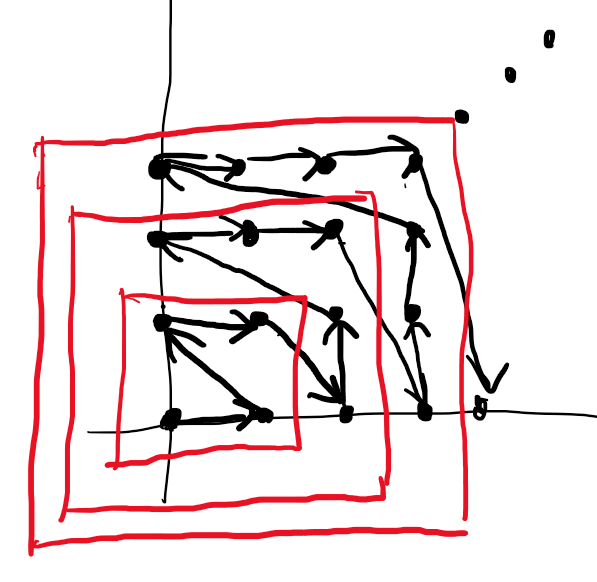
\includegraphics[width=0.4\linewidth]{winding.png}
  \label{fig:test1}
\end{figure} 
It's clear that this defines a well ordering. The red squares indicate the key fact of importance regarding this, which is that for any $(\alpha,\beta) \in \kappa \times \kappa$, the entire initial segment given by this point is bounded inside of the box $\max\{\alpha,\beta\} \times \max\{\alpha,\beta\}$, which by induction has cardinality at most $\max\{\alpha,\beta\} < \kappa$. Thus, all proper initial segments of $\kappa \times \kappa$ are order-isomorphic to an ordinal of cardinality smaller than $\kappa$. If we let $f(\alpha,\beta)$ map to the ordinal isomorphic to that initial segment then, we will get a mapping from $\kappa \times \kappa$ to $\kappa$, one which is clearly a bijection. 
\end{proof}
\begin{theorem}[Cantor]
	For any set $X$, there does not exist a surjective map from $X$ onto $\mathcal{P}(X)$. 
\end{theorem}
\begin{proof}
	Suppose $f: X \to \mathcal{P}(X)$ were onto. Define $\bar{D} \subseteq X$ by $\bar{D} = \{x \in X: x \notin f(x)\}$. Now, $\bar{D}$ is a subset of $X$, so it has to equal $f(d)$ for some $d \in X$, i.e. $f(d) = \bar{D}$. Now, if $d \in f(d) = \bar{D}$, then by definition of $\bar{D}$ it follows that $d \notin f(d)$, contradiction. Thus it must be that $d \notin f(d)$. But then it immediately follows that $d \in \bar{D}$, a contradiction again. Thus it must be that $f$ is not onto, contradiction. 
\end{proof}
\begin{definition}
Let $\alpha$ be a limit ordinal. The \textbf{cofinality} of $\alpha$, denoted $cof(\alpha)$, is the least ordinal $\beta$ such that there is a function $f:\beta \to \alpha$ which is \textit{unbounded}, or \textbf{cofinal} in $\alpha$, in the sense that for all $\alpha' < \alpha$, there exists a $\beta' < \beta$ such that $f(\beta) \geq \alpha'$. 
\end{definition}


\par \textbf{Infinity} \[\exists x (\varnothing \in x \wedge \forall y (y \in x \rightarrow y \cup \{y\} \in x)) \]The infinity axiom asserts that there exists a set $x$ which contains the empty set, and furthermore that is closed under the successor function.
\par \textbf{Power Set} \[\forall x \exists y \forall z (z \subseteq x \rightarrow z \in y) \]
	Here $x \subseteq y$ abbreviates \[\forall w (w \in z \rightarrow w \in x)\] 

	The idea here is that $z$ is a universe of discourse, $\phi(w_1,...,w_n)$ is some parameter, and $y$ is the set $\{x \in z: \phi(w_1,...,w_n)\}$. So it is the axiom which allows us to define sets in the way most are comfortable with.
\par \textbf{Foundation}
	\[ \forall x [((\exists y)y \in x) \rightarrow (\exists y(y \in x \wedge \neg \exists z (z \in x \wedge z \in y)))] \]
	This axiom specifies that every nonempty set contains a set which is disjoint from the set itself.
\begin{lemma}
	There exists an empty set. That is to say, $ZF \vdash \exists x \forall y (\neg (y \in x))$
\end{lemma}
\begin{proof}
	First, note that $ZF$ proves that sets exist:  is a basic logical axiom,  Next, note by composition that if we let $\phi(x,z) = (x \neq x) \wedge (x \in z)$, then by comprehension we have that $ZF \vdash \forall z \exists y \forall x (x \in y \leftrightarrow (x \in z \wedge \phi(x,z))$, from which it clearly follows by simplification of the inside statement and use of the logical axiom $\forall x \phi \rightarrow \phi_t^x$ we get that $ZF \vdash \exists z(z = z) \wedge \exists y \forall x (x \in y \leftrightarrow (x \in y \leftrightarrow (x \in z \wedge x \not\approx x)))$. Clearly the set $y$ here is the empty set. Uniqueness of this set follows from extensionality.  
\end{proof}


\begin{theorem}[Set Transfinite Recursion Theorem]
Do
\end{theorem}
\begin{definition}
	For $\alpha \in ON$, the set $V_{\alpha}$ is defined by transfinite recursion as follows:
	\begin{itemize}
		\item[1] $V_0 = \varnothing$.
		\item[2] For $\alpha+1$ a successor ordinal, $V_{\alpha+1} = \mathcal{P}(V_{\alpha})$
		\item[3] For $\alpha$ a limit ordinal, $V_{\alpha} = \bigcup_{\beta < \alpha} V_{\beta}$. 
	\end{itemize}
	This sequence of collections of sets is known as the \textbf{rank hierarchy}.
\end{definition}
\begin{lemma}
	For all $\alpha \in ON$, $V_{\alpha}$ is transitive. If $\alpha < \beta$, then $V_{\alpha} \subseteq V_{\beta}$. 
\end{lemma}
\begin{proof}
	We show transitivity by induction on the ordinals. Trivially we of course have it for the case for $\alpha = 0$. Suppose $x \in y \in V_{\alpha+1}$ for $\alpha+1$ a successor ordinal. Then since $V_{\alpha+1} = \mathcal{P}(V_{\alpha})$, it must be the case that $y \subseteq V_{\alpha}$, meaning that $x \in V_{\alpha}$. By inductive hypothesis $V_{\alpha}$ is transitive, meaning that for all $z \in x \in V_{\alpha}, z \in V_{\alpha}$, which leaves us with $x \subseteq V_{\alpha}$, which leaves us with $x \in V_{\alpha+1}$. Since a union of transitive sets is transitive, we have that $V_{\alpha}$ is transitive in the limit case via the definition. This completes the induction. \par 
	Towards the second claim, we again go by induction on $\beta$ for all $\beta \geq \alpha$. For $\beta = \alpha$ this is trivial. Again the limit ordinal case is trivial by the definition and the inductive hypothesis. Suppose $\beta+1$ is a successor ordinal. Want to show $V_{\alpha} \subseteq V_{\beta+1}$. Clearly if we have the limit case, then it is enough to show that $V_{\beta} \subseteq V_{\beta+1}$. If $x \in V_{\beta}$, then by transitivity all $z \in x$ are also in $V_{\beta}$, so $x \subseteq V_{\beta}$, and thus $x \in V_{\beta+1}$, the desired result.
\end{proof}
So this is indeed a hierarchy - an ascending sequence. 
\begin{definition}
	Let $x$ be a set. First, for $n \in \omega$, define $\bigcup^n(x)$ recursively by $\bigcup^0(x) = x$, $\bigcup^{n+1}(x) = \bigcup\left(\bigcup^n(x)\right)$. Define the \textbf{transitive closure} of $x$ by $trcl(x) = \bigcup_{n \in \omega} \left( \bigcup^n(x) \right)$. 
\end{definition}
It should be clear that $trcl(x)$ is the smallest transitive set containing $x$. The next lemma gives us that every set can be found somewhere in this hierarchy. (Provided we have an actual model of $ZF$.)
\begin{lemma}
	For every $x$ there is an $\alpha \in ON$ such that $x \in V_{\alpha}$. 
\end{lemma}
\begin{proof}
	Suppose not, and fix an $x$ not in any $V_{\alpha}$. Let $y = trcl(\{x\})$, and then let $s = \{z \in y: z \notin \bigcup_{\alpha \in ON} V_{\alpha}\}$. This has to be a set by comprehension, and is nonempty since at the very least $x \in s$ (this is why we let $y = trcl(\{x\})$ instead of just $y = trcl(x)$. Since $s$ is nonempty, it has an $\in$-minimal element, call it $z$. That is to say, $z \in s \subseteq y$ has the property that nothing inside of it is also in $s$. Now $z \in y$ and $y$ is transitive, meaning that $z \subseteq y$. This isn't a contradiction yet - the contents of $z$ could all exist in $y-s$. Note that by minimality of $z$ within $s$, it has to be the case that for all $w \in z, w \in V_{\alpha}$ for some $\alpha$. By replacement then we can define a set of ordinals such that for each $w \in z$, $w$ is in at least one of the associated $V_{\alpha}$, and then by the union axiom we can take the union of these ordinals, which is itself an ordinal, call it $\alpha$. Then it is clear that all $w \in z$ are also in $V_{\alpha}$, meaning that $z \subseteq V_{\alpha}$, meaning that $z \in V_{\alpha+1}$, a contradiction.
\end{proof}
This assurance that, at least for models of $ZF$, the rank hierarchy contains every set in the model, we can make the following definition which in some sense classifies the complexity of sets.
\begin{definition}
	Define the \textbf{rank} of a set $x$ to be the least $\alpha \in ON$ such that $x \subseteq V_{\alpha}$. Note that this is a subset and not membership. Thus $rank(x)$ is defined to be $\alpha$ iff $V_{\alpha+1}$ is the least element of the rank hierarchy in which $x$ appears. 
\end{definition}
The rank hierarchy is useful because it allows us to prove facts about all sets in a model via induction, by inducting on the rank hierarchy. 
\section{Absoluteness}
	We want to speak about the truth value of certain statements remaining true across different models, in particular with the language of set theory, and more particularly with extensions of models. A model for set theory is defined by only two things: a set $M$ (or class), and a relation $E$ (or class function) which represents set membership. Within first order logic, given a formula $\phi(x_1,...,x_n)$, and $a_1,...,a_n \in M$, we understand fully well what the statement $M \models \phi(a_1,...,a_n)$ means. What we would like to do now is take the discussion of first order logic and \textit{embed it} inside of a particular model of set theory. That is to say, within some model of set theory, we will have a set (or class) $M$, and a relation (or class relation) $E$, and we would like to find a formula $\phi^{(M,E)}$ which \textit{represents} the statement that $(M,E) \models \phi(a_1,...,a_n)$. We will denote this statement $\phi^{(M,E)}$ and call it the \textbf{relativization} of $\phi$ to $(M,E)$. 
	\begin{definition}
		Let $M,E$ be classes, and $\phi$ a formula in the language of set theory. We define $\phi^{(M,E)}$ by induction on $\phi$ through the following cases.
		\begin{itemize}
			\item[(1)]
				$(x \in y)^{(M,E)} = (xEy)$
			\item[(2)]
				$(x \approx y)^{(M,E)} = (x \approx y)$
			\item[(3)]
				$(\exists x \psi)^{(M,E)} = \exists x\in M(\psi^{(M,E)})$
			\item[(4)]
				$(\neg \psi)^{(M,E)} = \neg(\psi^{(M,E)})$. 
		\end{itemize}
	\end{definition}
If $E$ is the $\epsilon$ relation, or if $E$ is understood, we simply write $\phi^M$. Note that if $M$ and $E$ are sets, then $\phi^{(M,E)}$ is going to be a formula with parameters, namely the sets $M$ and $E$. Whereas if $M$ and $E$ are pure classes (i.e. given by formulas) then $\phi^{(M,E)}$ will be a formula in the language of set theory (i.e. without parameters). The following should be clear, as this was the point of the definition:
\begin{fact}
	For all sets $M,E$, formulas $\phi(x_1,...,x_n)$ and $a_1,...,a_n \in M$, $\phi^{(M,E)} \iff (M,E) \models \phi(\vec{a})$. 
\end{fact}
\begin{definition}
	Let $\phi(x_1,...,x_n)$ be a formula in the language of set theory. Let $M \subseteq N$ be sets or classes. Let $E \subseteq N \times N$ be a set or class, and let $E' = E \cap (M \times M)$. We say that $\phi$ is \textbf{absolute} between $M$ and $N$ if for all $a_1,...,a_n \in M$, we have $\phi^{(M,E')}(a_1,...,a_n) \iff \phi^{(N,E)}(a_1,...,a_n)$.  
\end{definition}
Thus a formula is absolute if, when 'extending our model to something bigger', it remains true provided it was true in the original model. Note that in the above definitions, there is quite a bit of generality in a few senses. Our sets and relations have no obligation to actually be a model of and theory, and they are allowed to be parameterized. For example, if we let $N = \omega$, and $M \subseteq N$ be the odd numbers, and consider the formula $\phi(x) = \exists y (y \in x)$, then this is actually abolute between $M$ and $N$, despite it not being true in general for $N$. Next we restate the definition of the following familiar hierarchy in the context of the language of set theory.
\begin{definition}
	A formula in the language of set theory is $\Delta_0$ if it is in the smallest collection satisfying the following:
	\begin{itemize}
		\item[(1)]
			All atomic formulas are $\Delta_0$
		\item[(2)]
			If $\phi,\psi \in \Delta_0$, then so are $\neg \phi, \phi \wedge \psi,\phi \vee \psi$. 
		\item[(3)] If $\phi(x_1,...,x_n) \in \Delta_0$, then so are $\psi(x_1,...,x_n) = \exists y \in \{x_i\} \phi(x_1,...,x_n,y)$ and $\psi(x_1,...,x_n) = \forall y \in \{x_i\} \phi(x_1,...,x_n,y)$
	\end{itemize}
	A formula is said to be $\Sigma_n$ if it is logically equivalent to a formula of the form $\exists x_1...\exists x_n \phi$ (should be $m$ for the number of quantifiers? like general m?) where $\phi \in \Pi_{n-1}$, and said to be $\Pi_n$ if it is logically equivalent to one of the form $\forall x_1...\forall x_n \phi$ where $\phi \in \Sigma_{n-1}$. 
\end{definition}
\begin{lemma}
	Let $(M,E') \subseteq (N,E)$ where $M,N,E$ are sets or classes, and $E' = E \cap (M \times M)$. Assume that whenever $a \in M$, $b \in N$, and $bEa$, then $b \in M$ (i.e. if $E$ were the actual $\in$ relation, we would be saying that $M$ is transitive). Then any $\Delta_0$ formula is absolute between $(M,E')$ and $(N,E)$. 
\end{lemma}
\begin{proof}
	By induction on the formula $\phi$. Beginning with the atomic cases, if $\phi = (x \approx y)$, then simply noting that by definition $(x \approx y)^{(M,E)} = (x \approx y)$ is independent of $M$ and $E$, it is obvious that $\phi$ is absolute between $M$ and $M$. For the case $\phi = (x \in y)$, suppose $x,y \in M$. If $(x \in y)^{(M,E')}$, then $xE'y$, so obviously $xEy$, meaning that $(x \in y)^{(N,E)}$. Conversely if $(x \in y)^{(N,E)}$, then $xEy \implies xE'y \implies (x \in y)^{(M,E')}$, so we have absoluteness for membership. 
	\par Turning to our inductive step, we note that the case of Boolean connectives is trivial. Next we consider $\phi(x) = \exists y \in x \psi(x,y)$ (i.e. $\exists y (y \in x \wedge \psi(x,y))$. Let $a \in M$. If $\phi^{(M,E')}(a)$ then by our definition this means $(\exists b(b \in a \wedge \psi(a,b)))^{(M,E')} \implies \exists b [b \in M \wedge (b \in a \wedge \psi(a,b))^{(M,E')})] \implies \exists b [b \in M \wedge (bE'a \wedge \psi^{(M,E')}(a,b))]$. But of course $bE'a \implies bEa$, and $\psi^{(M,E')}(a,b) \implies \psi^{(N,E)}(a,b)$ by induction, and so this statement implies $\exists b [b \in M \wedge (bEa \wedge \psi^{(N,E)}(a,b))] \implies \exists b[b \in M \wedge (b \in a \wedge \psi(a,b))^{(N,E)}] \implies \phi^{(N,E)}(a)$. Conversely, suppose $\phi^{(N,E)}(a)$, that is to say, $\exists b(b \in a \wedge \psi(a,b)))^{(N,E)}$. Then $\exists b [b \in N \wedge (b \in a \wedge \psi(a,b))^{(N,E)}] \implies \exists b [b \in N \wedge (bEa \wedge \psi^{(N,E)}(a,b))]$. But then $b \in N$ and $b \in a$ means that $b \in M$ by hypothesis, and so of course also $bE'a$ and so we have $\exists b [b \in M \wedge (bE'a \wedge \psi^{(M,E')}(a,b))] \implies \exists b [b \in M \wedge (b \in a \wedge \psi(a,b))^{(M,E')}] \implies \phi^{(M,E')}(a)$. 
\end{proof}
\begin{corollary}
	If $M \subseteq N$ are sets and $E$ is the $\in$ relation, and $M$ is transitive, then any $\Delta_0$ formula is absolute between $M$ and $N$.
\end{corollary}
Note that what we proved above was actually stronger than what we needed to prove - there was no need anywhere to assume that the set we were quantifying over was bounded. This contributes to the next result:
\begin{lemma}
	Let $(M,E') \subseteq (N,E)$ satisfy the hypotheses of the above lemma. Then if $\phi(\vec{x}) \in \Sigma_1$ and $\phi^{(M,E')}(\vec{a})$ for some $\vec{a} = a_1,...,a_i \in M$, then $\phi^{(N,E)}(\vec{a})$. 
\end{lemma} 
\section{Forcing}
\begin{definition}
	A \textbf{partial order} is a set $P$ together with a reflexive, transitive binary relation $\leq$, i.e. $\mathbb{P} = < P, \leq > $. Sometimes we will assume that a partial order has a largest element, denoted $\mathbb{1}$. For $p,q \in P$, we say that $p$ and $q$ are \textbf{compatible}, and write $p || q$, if there exists an $r \in P$ such that $r \leq p$, and $r \leq q$. Otherwise we say they are \textbf{incompatible}, and write $p \perp q$. 
\end{definition}
\begin{definition}
	We say that a set $A \subseteq P$ is an \textbf{antichain} if it's elements are all pairwise incompatible. An antichain $A$ is \textbf{maximal} if every $p \in P$ is compatible with some $a \in A$. We say that a set $D \subseteq P$ is \textbf{dense} if $\forall p \in P, \exists q \in D$ such that $q \leq p$. We say a set $V$ is \textbf{predense} if $\forall p \in P,\exists q \in V$ such that $(q || p)$. Note that if a set $V$ is predense, then if we define $D = \{p \in P: p \leq v \textrm{ for some } v \in V \}$, which we refer to as the \textbf{downward closure} of $D$, then $D$ is dense, since for all $p \in P$, predenseness implies there is a $q \in V$ such that $q \leq p$, but then $q \in D$, meaning we always have a $q \in D$ such that $q \leq p$ for any $p \in P$.
\end{definition}
\begin{definition}
	A \textbf{filter} $G$ on a partial order $\mathbb{P}$ is a subset $G \subseteq P$ such that for all $p,q \in G$, $p||q$, and for all $p \in G$, we have that for all $q \geq p$, $q \in G$. So elements of a filter must be compatible, and $G$ itself must be closed upward. Note that just because $G \subseteq P$ does not mean that $G \in M$!!!!
\end{definition}
Let $(X,\tau)$ be a topological space, and note that $(\tau,\subseteq)$ is always a partial order. If $D \subseteq \tau$ is dense in the above sense, then if we choose a single element $x$ out of each $V \in D$, we will have a dense set in the topological sense. Also, filters in the above sense are precisely filters in the typical set theoretical sense. 
\begin{definition}
	Let $M$ be a model of $ZF$ (some universe of discourse), and let $\mathbb{P} \in M$ be a partial order. Then an \textbf{$\bm{M}$-generic} is a filter $G$ over $\mathbb{P}$ which has a nonempty intersection with any dense set $D \subseteq P$. 
\end{definition}
\begin{fact}
	$G$ is an $M$-generic iff $G$ meets all of the predense sets $V \subseteq P$ iff $G$ meets all maximal antichains $A \subseteq P$. 
\end{fact}
\begin{proof}
	Suppose that $V$ is predense. If $G$ is an $M$-generic, then $G$ has to meet the set $D = \{p \in P: p \leq q \textrm{for some } q \in V\}$. Let $p \in G \cap D$. Then since $p \in D$, there is a $d \in D$ such that $d \leq p$, but this means there is a $q \in V$ such that $d \leq q$. But since $G$ is a filter and filters are closed upwards, we must have that $q \in G$, and so $q \in G \cap V$, and so $G$ meets arbitrary predense sets. Obviously the converse is true - if $G$ meets all predense sets, then since all dense sets are also predense, we have immediately that $G$ meets all dense sets as well. \par
	Next we claim that all maximal antichains are predense. Consider the downward closure $D$ of a maximal antichain $A$. Let $p \in P$, then since $A$ is maximal there must be an $a \in A$ such that $a || p$, i.e. there is a $q \in P$ such that $q \leq a$, and $q \leq p$, but $q \leq a \implies q \in D$, and so for this arbitrary $p$ we've found a $q \in D$ such that $q \leq p$, i.e. $D$ is dense. Thus all maximal antichains are predense and so if $G$ is an $M$-generic, it meets all predense sets and thus must meet all maximal antichains as well. \par 
	Finally, suppose that $G$ meets all maximal antichains. Suppose that $V$ is predense. Clearly this doesn't need to be an antichain, but we can thin it out into an antichain, and it's predenseness will force it to be maximal. Suppose that $p,q \in V$ are compatible. We claim that we can throw out $q$ and still have a predense set. [need to finish]
\end{proof}
\begin{fact}
	If $A$ is dense below $p$, then any generic containing $p$ will meet $A$. 
\end{fact}
\begin{proof}
	By dense below $p$, it must be meant that for all $q \leq p$, there exists an $r \in A$ such that $r \leq q$. Suppose $G$ is a generic containing $p$. Want to show that $G \cap A \neq \varnothing$. 
\end{proof}
\begin{definition}
	A partial order $\mathbb{P}$ is \textbf{splitting} if for all $p \in P$, there exists a $q \leq p$ and an $r \leq p$ such that $q \perp r$. 
\end{definition}
\begin{lemma}
	If $G$ is an $M$-generic for $\mathbb{P}$, and $p \in P$ is compatible with every point in $G$, then there exists a $q \in G$ such that $q \leq p$. 
\end{lemma}
\begin{proof}
	Let $G$ and $p$ be as above. Let $D = \{q \in P: (q \perp p) \vee (q \leq p) \}$. We claim that $D$ is dense. To see this, let $l \in P$ be arbitrary. Either $l \perp p$ or $l || p$. In the former case, we obviously have that $l \in D$, and since $l \leq l$, we have $l$ as it's own representative to observe denseness. On the other hand, $l ||p$ means there is an $r \in P$ with $r \leq p$ and $r \leq l$. But $r \leq p$ means that $r \in D$, and so $r$ observes denseness. This shows that $D$ is dense. Now since $G$ is a generic, $G \cap D$ is nonempty - let $q$ be an element of this intersection. Since $q \in G$, by hypothesis we must have that $p ||q$, but this means that it cannot be the case that $p \perp q$, and so we must conclude that $q \leq p$, completing the proof. 
\end{proof}
\begin{lemma}
	If $M$ is a transitive model of $ZF$, $\mathbb{P} \in M$, $\mathbb{P}$ is splitting, and $G$ is an $M$-generic for $\mathbb{P}$, then $G \notin M$. 
\end{lemma}
\begin{proof}
	Suppose by way of contradiction that $G \in M$. Consider $D = \{p \in P: p \perp q \textrm{ for some }p \in G\}$. We claim $D$ is dense. Fix a $p \in P$. Since $\mathbb{P}$ is splitting, there exists a $q,r \in P$ such that $q \leq p$ and $r \leq p$ and $q \perp r$. We claim that at least one of these is in $D$. If this is the case, say it's $q$, then $q \in D$ is such that $q \leq p$, so $D$ is dense, but then we have a contradiction because, since $G$ is generic, $G \cap D$ is nonempty, so if we pick $l \in G \cap D$, then since $l \in D$, there exists an $r \in G$ such that $q \perp r$, contradicts $G$ being a filter (we've found two elements which are incompatible). Towards showing that at least one of $q,r \in D$, note that this means that for all $l \in G$, $ l||q$ and $l||r$. Thus pick any $l$, and then there must exist a $q',r'$ such that $q',r' \leq l$, $q' \leq q$, and $r' \leq r$. Since $G$ is a filter, $q'||r'$, and so there exists an $s \in P$ such that $s \leq q'$ and $s \leq r'$. But then by transitivity $s \leq q$ and $s \leq r$, meaning that $q ||r$, contradicting that $q \perp r$. This completes the proof. 
\end{proof}
\begin{lemma}
	Let $M$ be a countable model of $ZF$, and $\mathbb{P} \in M$. Then there exists an $M$-generic filter for $P$.
\end{lemma}
\begin{proof}
	Since the model is countable we can enumerate the dense subsets of $P$ which lie in $M$, $D_0,D_1,D_2,...$. Pick any $p_0 \in D_0$. Then by denseness of $D_1$, we can pick a $p_1 \leq p_0$ in $D_1$, and so forth, to construct the decreasing sequence $p_0 \geq p_1 \geq p_2 \geq \ldots$. Let $G = \{p \in P: p \geq p_n \textrm{ for some }n \in \mathbb{N}\}$. We claim that $G$ is a filter. First, if $q,r \in G$, then $\exists m,n$ such that $q \geq p_n$, $r \geq p_m$. WLOG let $n\geq m$, and so $p_m \leq$ both $q$ and $r$, meaning that $q||r$. Next, if $q \in G$ and $r \geq q$, then since $q \geq p_n$ for some $n$, so is $r$ by transitivity, meaning that $r \in G$, meaning that $G$ is a filter. Finally, let $D$ be arbitrary, dense. Then $D = D_n$ for some $n \in \mathbb{N}$, and namely $p_n \in D_n$ with $p_n \geq p_n$, meaning that $p_n \in G$, so $p_n \in G \cap D_n$, meaning $G$ is a generic.
\end{proof}
\begin{definition}
	Let $M$ be a model of $ZF$, and $\mathbb{P} \in M$ a partial order. By transfinite recursion on $ON^M$ we define $M_{\alpha}^{\mathbb{P}}$ as follows: $M_0^{\mathbb{P}} = \varnothing$. For $\alpha$ a limit ordinal, $M_{\alpha}^{\mathbb{P}} = \bigcup_{\beta < alpha}M_{\beta}^{\mathbb{P}}$. We define $\tau \in M_{\alpha+1}$ iff $\tau \in M_{\alpha}$ or $\tau$ is a relation with $dom(\tau) \subseteq M_{\alpha}$ and $ran(\tau) \subseteq P$. We let $M^{\mathbb{P}} = \bigcup_{\alpha \in ON^M}M_{\alpha}^{\mathbb{P}}$. We call these $\tau$ \textbf{names}
\end{definition}
Thus a name $\tau$ is a set of ordered pairs $(\sigma,p)$ where $\sigma$ is a name of smaller rank and $p \in P$. Effectively, we are constructing a duplicate universe of sets, but with elements of $p$ tagged with elements of the partial order $P$. The names within the set $M^{\mathbb{P}}$ are effectively symbols which represent a copy of $M$. However we would also like to represent the elements of $M$ itself, which we do in the following way. Note that for every object that would normally be a set in the rank hierarchy, that single set is paired with \textit{every} subset of $P$. 
\begin{definition}
	Again by transfinite recursion in $M$, define for each $x \in M$ the name $\check{x}$ by $\check{x} = \{<\check{p},p>: y \in x \wedge p \in P\}$. Also, define $\dot{G}$ by $\dot{G} = \{<\check{p},p>: p \in P \}$.  
\end{definition}
These things are just symbols currently. It is through the additional object, a filter, $G$, by which we create what are effectively new models of $M$.
\begin{definition}
	Let $M$ be a model of $ZF$, and $\mathbb{P} \in M$ a partial order. Let $G \subseteq P$ be a filter. For $\tau \in M^{\mathbb{P}}$, define $\tau_G$ by transfinite recursion via $\tau_G = \{\sigma_G: \exists p \in G \textrm{ such that }<\sigma,p> \in \tau\}$. Finally, for a filter $G$ on $P$, define $M[G]$ to be the set of all names, evaluated according to $G$.
\end{definition}
Note that $\tau_{G}$ is obtained by 'plucking' appropriate names names out of their paired point in $P$ according to whether or not that point is in the filter $G$. A quick induction on the rank hierarchy confirms that for all $x \in M$, $\check{x}_G = x$, and from this it follows that for any filter $G$, $(\dot{G})_G = G$, meaning that $G \in M[G]$. From this we have the following important facts about $M[G]$ which justify the construction.
\begin{lemma}
	It's always the case that for any model $M$ of $ZF$, any partial order $\mathbb{P} \in M$, and any filter $G$ over $\mathbb{P}$, $M \subseteq M[G]$, with $G \in M[G]$. Moreover if $\mathbb{P}$ is splitting, $M$ is transitive, and $G$ is an $M$-generic, then $G \notin M$.
\end{lemma}
We next want to find conditions which ensure that $M[G]$ is a model of $ZF$, and find a way to relate truth in $M[G]$ to truth in $M$. Towards this we begin with the following:
\begin{lemma}
	$M[G]$ is transitive and $ON^{M[G]} = ON^{M}$.
\end{lemma}
\begin{proof}
	If $x \in M[G]$, then $x = \tau_G$ for some $\tau \in M^{\mathbb{P}}$. If $y \in x$, then by definition of $\tau_G$ it follows that $y = \tau_G$ for some $\tau \in M^{\mathbb{P}}$, so $y \in M[G]$. Thus $M[G]$ is transitive. [Still need to do claim about ordinals]
\end{proof}
\begin{lemma}
	Any transitive set satisfies the foundation and extensionality axioms
\end{lemma}
From this and a bit more argumentation we get $4$ of the $ZF$ axioms for $M[G]$. For the other half, we will need to prove the forcing theorem.
\begin{lemma}
	If $M$ is a transitive model of $ZF$, then for any filter $G$, $M[G]$ satisfies the extensionality, pairing, union, and foundation axioms.
\end{lemma}
	\begin{proof}
	todo
\end{proof}
\begin{definition}
	By the \textbf{forcing language} we mean all statements of the form $\phi(\sigma_1,...,\sigma_n)$ where $\phi(x_1,...,x_n)$ is a formula in the language of set theory and $\sigma_1,...,\sigma_n \in M^{\mathbb{P}}$. \par 
	For a $p \in \mathbb{P}$, we proceed to define the notion of $p$ \textbf{forcing} $\phi(\sigma_1,...,\sigma_n)$, denoted $p \Vdash \phi(\sigma_1,...,\sigma_n)$. This will be done via a combination of induction and transfinite recusion: for atomic $\phi$ it is defined by transfinite recursion in $M$, on the maximum of the ranks of the $\sigma_i$. The induction will follow from there in the standard way. Note that the following definition takes place \textit{entirely in M}, in the sense that there is a class function from $M^{\mathbb{P}}$ to $\mathbb{P}$ which assigns to each $(\sigma_1,...,\sigma_n) \in (M^{\mathbb{P}})^n$ the set $\{p \in P: p \Vdash \phi(\sigma_1,...,\sigma_n)\}$.  
	\par Let $M$ be a transitive model of $ZF$ and $\mathbb{P}$ a partial order in $M$. For $p\in P$ and $\phi(\sigma_1,...,\sigma_n)$ in the forcing language, the relation $p \Vdash \phi(\sigma_1,...,\sigma_n)$ is defined as follows:
	\begin{itemize}
		\item For $\phi = (\tau_1 \in \tau_2)$, define 
		\[ p \Vdash (\tau_1 \in \tau_2) \iff \{q \in P:(\exists \langle\sigma,r\rangle \in \tau_2)(q \leq r \wedge q \Vdash (\tau_1 \approx \sigma)) \} \textrm{ is dense below }p \]
		\item For $\phi = (\tau_1 \approx \tau_2)$, we say $p \Vdash \phi$ iff for all $\langle \sigma_1,q \rangle \in \tau_1$, the set
		\[ \{r: r \leq q \implies \exists \langle \sigma_2,s \rangle \in \tau_2(r \leq s \wedge r \Vdash (\sigma_1 \approx \sigma_2)   \} \]
		is dense below $p$ \textit{and} likewise for all $\langle \sigma_2,q \rangle \in \tau_2$ the set
		\[ \{r: r \leq q \implies \exists \langle \sigma_1,s \rangle \in \tau_1 (r \leq s \wedge r \Vdash (\sigma_1 \approx \sigma_2) \} \]
		is also dense below $p$.
		\item For $\phi = (\alpha \wedge \beta)$, we say that $p \Vdash \phi$ iff $p \Vdash \alpha$ and $p \Vdash \beta$. 
		\item For $\phi = \neg \psi$, we say that $p \Vdash \phi$ iff $\neg \exists q \leq p (q \Vdash \psi)$. 
		\item For $\phi(\sigma_1,...,\sigma_n) = \exists x \psi(\sigma_1,...,\sigma_n,x)$ we define $p \Vdash \exists x \psi (\sigma_1,...,\sigma_n,x)$ iff 
		\[ \{ q: \exists \tau \in M^{\mathbb{P}} q \Vdash \psi(\sigma_1,...,\sigma_n,\tau)\} \] is dense below $p$ 
	\end{itemize}
\end{definition}
This definition is extremely complicated, and solely exists for the following theorem, which we need a few lemmas to prove but will state now:
\begin{theorem}[The Forcing Theorem]
	Let $M$ be a countable, transitive model of $ZF$ and $\mathbb{P} \in M$ a partial order. We have the following:
	\begin{itemize}
		\item[(1)]
			For any $p \in P$ and $\sigma_1,...,\sigma_n \in M^{\mathbb{P}}$,
			\[ p \Vdash \phi(\sigma_1,...,\sigma_n) \iff \textrm{for all generics }G \textrm{ containing p }M[G] \models \phi((\sigma_1)_G,...,(\sigma_n)_G)  \]
		\item[(2)]
			For any generic $G$ and $\sigma_1,...,\sigma_n \in M^{\mathbb{P}}$, 
			\[ M[G] \models \phi((\sigma_1)_G,...,(\sigma_n)_G) \iff \exists p \in G (p \Vdash \phi(\sigma_1,...,\sigma_n) \]
	\end{itemize}
\end{theorem}
The forcing theorem is the key to relating our forcing notion within the model to truth in the larger model.
\begin{lemma}
\end{lemma}
Need to talk about partial orders equivalent for forcing via dense embeddings \par
For what follows, by \textbf{partial function} from $A$ to $B$ we mean a relation which would be a function if not for the fact that the domain is not necessarily all of $A$.  
\begin{definition}
	The \textbf{Cohen forcing} is the partial ordering $\mathcal{P} = \langle 2^{<\omega},\leq \rangle$ in which $x \leq y$ is taken to mean that $x$ extends $y$. Alternatively, we can consider the partial functions $p:\omega \to \{0,1\}$ with finite support, again ordered by extension. 
\end{definition}
Since there is clearly a dense embedding from one of these to the other, they are equivalent ways to think about the forcing. A generic with respect to this forcing is known as a \textbf{Cohen real}. Technically, a generic $G \subseteq \mathcal{P}$ is not a real, but it can be identified as one. To show this, consider the set $D_n = \{p: n \in dom(p)\}$. This set is dense for each $n$: given a fixed $q \in \mathcal{P}$, if $n \in dom(p)$, then done, otherwise any function which extends $q$ up to that $n$ will do. If $G$ is generic, then $G \cap D_1 = \varnothing$, pick a $p$ in it, and begin to define the 'real' $x$ (real as in an element of Baire space) by $x(1) = p(1)$. Next, pick a $p \in G \cap D_2$ and define $x(2) = p(2)$, and so forth. Since all elements of $G$ are compatible, these functions all extend each other, so in fact we can simply define $x(n) = i$ iff there exists a $p \in G$ such that $p(n) = i$. Clearly, $M[G] = M[x]$ (why?), and henceforth we identify a generic with a corresponding real $x$. \par 
Fix a model $M$ of (enough of) $ZF$, and let $\kappa$ be a cardinal in $M$. We want to not just add a single real, but lots of reals. To this end, we define $FN(\kappa \times \omega,2)$ to be the set of all partial functions from $\kappa \times \omega$ to $\{0,1\}$, which forms a partial order by extension, just like before. Of course, a function $F:\kappa \times \omega \to 2$ can be identified with a $\kappa$ sequence of functions $F_{\alpha}: \omega \to 2$. Just as above, the set $D_{\alpha,n} = \{p: (\alpha,n) \in dom(p)\}$ is always dense, and so we can define an indexed $\kappa$ sequence of reals $x_{\alpha}$ just as we defined the single $x$ above. We summarize these results along with one other important aspect below:
\begin{lemma}
	Let $M$ be a transitive model of $ZF$, $\kappa$ a cardinal of $M$, and $G$ an $M$-generic for $FN(\kappa \times \omega,2)^M$. Then $G$ can be identified with a function $G:\kappa \times \omega \to 2$. If $\{G_{\alpha}\}_{\alpha < \kappa}$ is the corresponding sequence of 'reals', then $G_{\alpha} \neq G_{\beta}$ if $\alpha \neq \beta$.  
\end{lemma} 
\begin{proof}
	We've already shown everything except that the reals are distinct. To see this, suppose that $\alpha \neq \beta$, and note that $D_{\alpha,\beta} = \{p: \exists n \in \omega (p(\alpha,n) \neq p(\beta,n)\}$ is always dense (we didn't also write the requirement that both $p$ is defined at both of these points, but that should be there too): given an arbitrary partial function $q: \kappa \times \omega \to 2$, we can easily find an extension $p$ which meets the required conditions (since we can always move as far 'down' each path as we need to in order to meet the 'end' of where $q$ is defined, hence the $\exists n \in \omega$. Thus choose $p \in G \cap D_{\alpha,\beta}$, and note that, indeed, $G_{\alpha}$ and $G_{\beta}$ must be different reals. 
\end{proof}
\begin{definition}
	A partial order $\mathcal{P}$ has the \textbf{countable chain condition}, or is said to be c.c.c., if every antichain $A \subseteq P$ is countable. More generally, $\mathcal{P}$ is said to be $\kappa$.c.c. if every antichain $A \subseteq P$ has size $<\kappa$. The \textbf{saturation}, or \textbf{cellularity} of $\mathcal{P}$, denoted $sat(\mathcal{P})$, is the least $\kappa$ such that $\mathcal{P}$ is $\kappa.c.c$. 
\end{definition}
\end{document}
